239. \begin{figure}[ht!]
\center{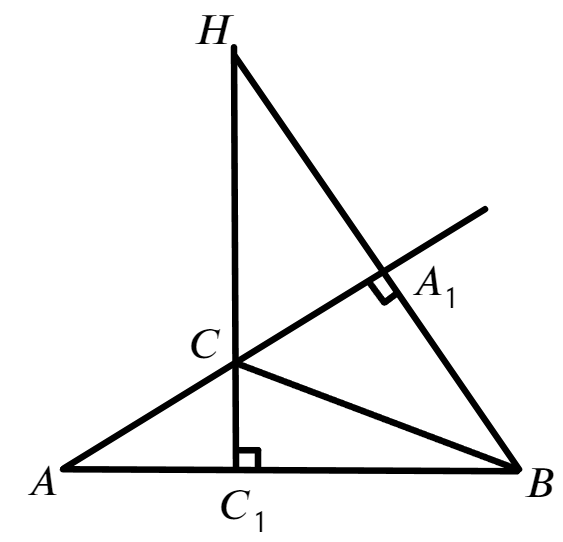
\includegraphics[scale=0.35]{g30-2.png}}
\end{figure}\\
Пусть высоты $AA_1$ и $CC_1$ пересекаются в точке $H.$ Углы $\angle ACC_1$ и $\angle HCA_1$ равны как вертикальные, поэтому $\angle A_1AB=90^\circ-\angle ACC_1=90^\circ-\angle HCA_1=\angle CHA_1.$ Тогда треугольники $AA_1B$ и $HA_1C$ равны по гипотенузе ($AB=CH$) и острому углу ($\angle A_1AB=\angle CHA_1$). Поэтому $CA_1=BA_1,$ и треугольник $A_1CB$ является прямоугольным и равнобедренным, значит $\angle A_1BC=\angle A_1CB=45^\circ,$ поэтому $\angle ACB=180^\circ-\angle A_1CB=180^\circ-45^\circ=135^\circ.$\\
